\documentclass[10.5pt, a4paper]{jsarticle}

\usepackage{fancybox}
\usepackage{listings, jlisting}
\usepackage[dvipdfmx]{graphicx, color}
\usepackage{here}

\title{技術レポート}
\author{島根大学 渡邉直樹}
\date{3月26日}

\begin{document}

\maketitle

\section{概要}
これはJavaアップレット上でリバーシを再現したプログラムである。
クリックした時に反転できる場合は反転し、そうでない場合は何もしない。
特徴として、コマが置ける場所は色が異なっていてわかりやすくなっている。
また、サイズは自由に変更できる。

\section{動機}
私はリバーシを作ろうと考えた理由はJavaの練習をするためです。
リバーシを制作する中で、条件分岐や繰り返し処理を多く使用すると考え、リバーシを選択しました。
また、盤面上でのクリック等、操作がシンプルでJavaアップレットでの再現ができそうだったのでリバーシを選択しました。

\section{説明}
\subsection{Mainクラス}

主にアップレットの操作とクリック時の処理を記す。

\subsubsection*{paint(Graphics):void}

Appletクラスからオーバーライドしたものであり、描写全般を行う。
主に、下部の勝敗等を示すテキストを表示する。
ボードやコマの表示は、別のメソッドを呼び出すことにより行う。

\subsubsection* {mouseClickedMotion(MouseEvent):void}

MouseListenerインターフェイスからオーバーライドしたものであり、マウスをクリックした時の処理を行う。
クリックした位置がボード上である場合、そのマスに置けるかどうかを判定する。
置ける場合はそのマスに置き、ターンを渡す。
そして、相手のターンで置けなかった場合は、もう一度自分のターンになる。
その時点で、自分がコマを置けない場合は終了する。

最後に再描画する。

\newpage

\subsection*{Reversiクラス}

主にリバーシにおける操作による処理を記す。

\subsubsection*{int[][] board}
現在の盤面を示した配列である。値が0の場合は何も置いていない、1の場合は黒のコマ、2の場合は白のコマを置く。

\subsubsection*{enablePlace(boolean):boolean}

置けるかどうか判定するマスを格納したリスト checkPlace に含まれるマスのみを判定する。
もともと、すべてのマスを判定していたが、処理効率の向上のため、リスト管理とした。

すべて置ける場合は true を返す。

\subsubsection*{enablePlace(int, int, boolean):boolean}

引数で指定されたマスに対して置けるかどうか判定する。

\begin{enumerate}
    \item 距離dの地点について調べる。
    \item もし、何もおいていない場合はその方向の判定は行わない。黒の場合はその方向の距離を記憶する。
    \item もし白の場合は、特に何もしない。
    \item すべての方向を調べたら、距離d+1の地点について1を繰り返す。
\end{enumerate}

\subsubsection*{reverseDisk(int, int):void}

指定されたマスに対して、enablePlaceメソッドで記憶された方向と距離がわかるので、board[][]を用いて、各方向に対して、コマを反転させていく。

\subsubsection*{getWinner():String}

勝敗を示す文字列を返す。countDisks[] により、コマの数が多いほうが勝利する。

\newpage

\section{参考画像}

\begin{figure}[htbp]
  \begin{center}
    \begin{tabular}{c}

      \begin{minipage}{0.33\hsize}
        \begin{center}
          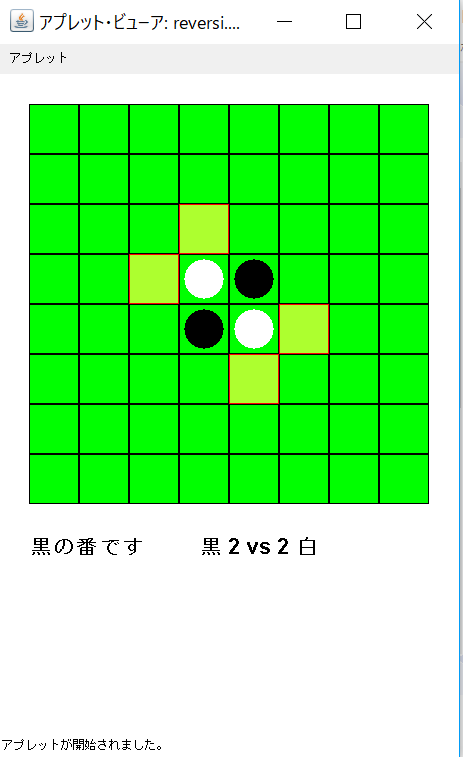
\includegraphics[clip, width=4.5cm]{./image/img01.png}
          \hspace{1.6cm} [1]初期画面
        \end{center}
      \end{minipage}

      \begin{minipage}{0.33\hsize}
        \begin{center}
          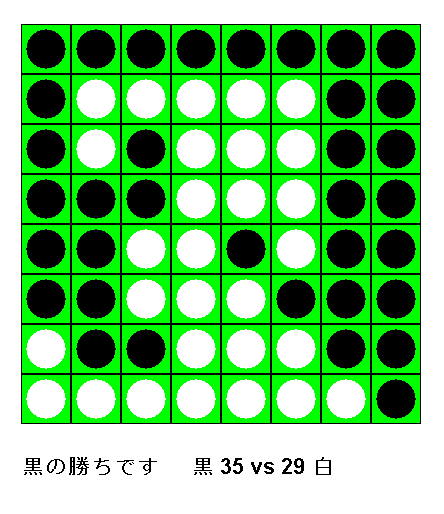
\includegraphics[clip, width=4.5cm]{./image/img02.png}
          \hspace{1.6cm} [2]黒が勝利
        \end{center}
      \end{minipage}

      \begin{minipage}{0.33\hsize}
        \begin{center}
          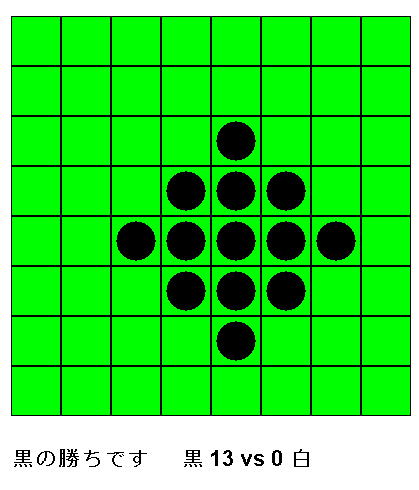
\includegraphics[clip, width=4.5cm]{./image/img03.png}
          \hspace{1.6cm} [3]黒が勝利
        \end{center}
      \end{minipage}

    \end{tabular}
  \end{center}
\end{figure}

\begin{figure}[htbp]
  \begin{center}
    \begin{tabular}{c}

      \begin{minipage}{0.33\hsize}
        \begin{center}
          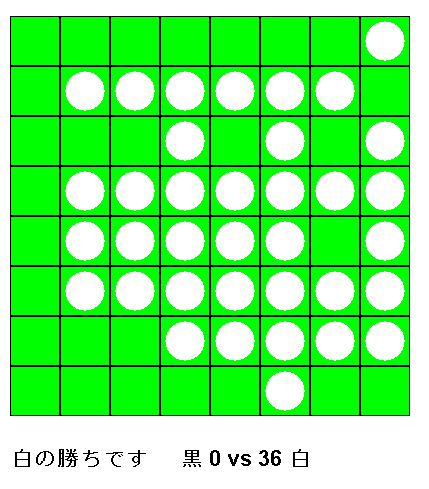
\includegraphics[clip, width=4.5cm]{./image/img04.png}
          \hspace{1.6cm} [4]白が勝利
        \end{center}
      \end{minipage}

      \begin{minipage}{0.33\hsize}
        \begin{center}
          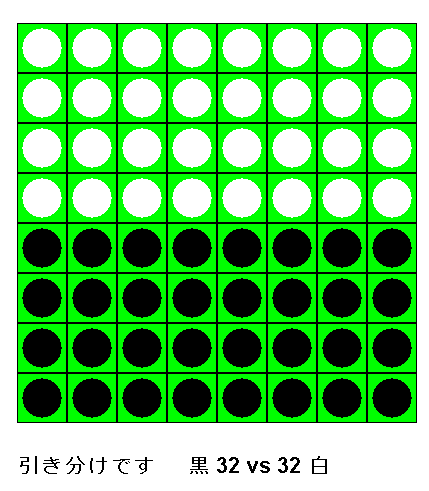
\includegraphics[clip, width=4.5cm]{./image/img05.png}
          \hspace{1.6cm} [5]引き分け
        \end{center}
      \end{minipage}

      \begin{minipage}{0.33\hsize}
        \begin{center}
          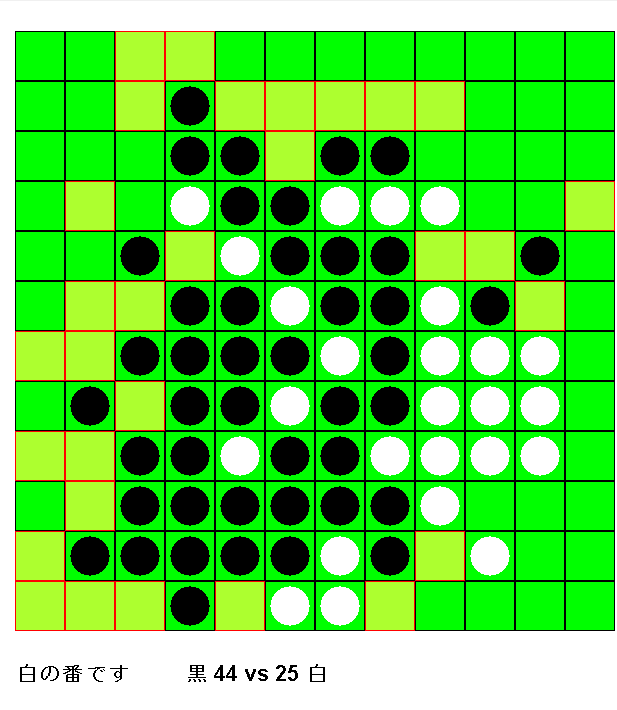
\includegraphics[clip, width=4.5cm]{./image/img06.png}
          \hspace{1.6cm} [6]サイズ変更
        \end{center}
      \end{minipage}

    \end{tabular}
  \end{center}
\end{figure}


\section{感想}
実際にJavaアップレットでリバーシを作成してみて、for文の範囲を設定する際、方向に応じて設定する範囲が異なり、難しく感じた。
処理内容をどちらのクラスに書くべきかを決めるのが大変だった。
しかし、完成した際には、最初に作ったものよりも段々と効率化していて、よりよいものができたのでよかった。
特に、リストを用いたことで置けるかどうかを判定する処理が格段に速くなったことに喜びを感じた。

\end{document}

